\chapter{Introduction : retour sur la non prise en compte de la densité par le Single-Linkage}
\rouge{10 avril - 15 avril}

Ce chapitre revient sur le problème fondamental du Single-Linkage : l'effet de chaînage, ou la non prise en compte de la densité locale.
Pourtant, si l'on voit le Single-Linkage dans l'espace euclidien comme on l'a fait dans la partie précédente : algorithme qui retrouve la hiérarchie exacte des amas de forte densité (modèle de \textsc{Hartigan}, voir \Def~\ref{def:high-density_clusters}~\&~\ref{def:HDC_discret}) pour l'estimateur de densité du $1$-NN, sa généralisation est claire :
\Citation{Il faut retrouver la hiérarchie exacte des amas de forte densité pour l'estimateur de densité des $K$ plus proches voisins ($K$-NN).}
Nous verrons sur un exemple simple pourquoi les généralisations proposées au problème dans la partie précédente ne marche. 
Nous verrons alors sur ce même exemple la véritable solution au problème.


\Contributions{Ce chapitre fait la transition entre l'introduction au Single-Linkage de la partie précédente, et la généralisation mathématiquement satisfaisante proposée dans les chapitres suivants. Nous espérons qu'elle fournisse au lecteur la bonne intuition pour que cette généralisation proposée dans les chapitres suivants lui paraisse effectivement naturelle.}



\section{L'échec du Robust Single-Linkage et de (H)DBSCAN sur le modèle de \textsc{Hartigan}}

Appelons $K\in \mathbb N^\star$ la variable représentant le nombre de voisins pris en compte dans l'algorithme de Robust Single-Linkage \cite{RobustSingleLinkage2010} et de (H)DBSCAN \cite{HDBSCAN, HDBSCAN2017}.
Pour $K = 1$, on a vu que le classique Single-Linkage fournissait exactement la hiérarchie des amas de forte densité dans le modèle de \textsc{Hartigan}.

En revanche, pour $K\ge2$, il n'y a plus correspondance entre la hiérarchie produite par ces algorithmes et celle du modèle (discret) de \textsc{Hartigan} (voir la fin du \S~\ref{chap:single-linkage_trois_vues}). 

Nous l'allons voir sur un exemple simple. Soit $\mathcal X = \bigl\{ A ; B ; C ; D ; E ; F\bigr\} \subset \mathbb R^2$ un nuage composé de six points disposés comme illustré en \Fig~\ref{fig:nuage} : deux triangles équilatéraux (de côté $2r$) parfaitement opposés et à distance $2r$ l'un de l'autre.


\begin{figure}[htbp]
    \centering
    
    % ---------------------------------------------------
    % SOUS-FIGURE (a) : Nuage de points X
    % ---------------------------------------------------
    \begin{subfigure}[b]{0.48\textwidth}
        \centering
        \begin{tikzpicture}[scale=0.6]
            
            % On définit le rayon r (la moitié de la longueur d'un segment)
            \def\r{1.5}
            
            % 1. Appel du template réutilisable
            \templateNuage[\r]
            
            % 2. Tracé des cercles en pointillés
            % (Les segments faisant 2r de long, les cercles sont magnifiquement 
            % tangents et se touchent au milieu parfait de chaque segment).
            \foreach \P in {A,B,C,D,E,F} {
                \draw[dashed, thick, gray] (\P) circle (\r);
            }
            
            % 3. Flèche pour faire apparaître visuellement le rayon r
            % On trace depuis A vers le haut-gauche (angle de 135 degrés).
            \draw[-, >=latex] (A) -- ++(135:\r) node[midway, sloped, above] {$r$};
            
        \end{tikzpicture}
        \caption{Niveau $r$}
        \label{fig:nuage}
    \end{subfigure}
    \hfill
    % ---------------------------------------------------
    % SOUS-FIGURE (b) : Dendrogramme sur X
    % ---------------------------------------------------
    \begin{subfigure}[b]{0.48\textwidth}
        \centering
        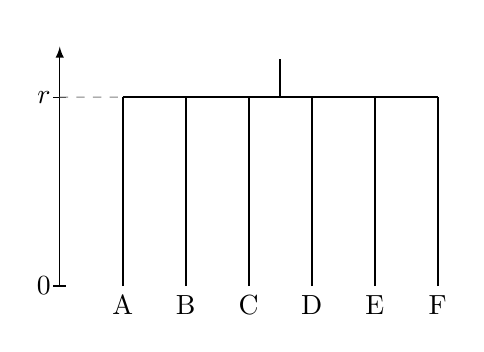
\begin{tikzpicture}[scale=0.8]
            
            % Les feuilles du dendrogramme (en bas de la figure)
            \coordinate (L1) at (0,0);
            \coordinate (L2) at (1,0);
            \coordinate (L3) at (2,0);
            \coordinate (L4) at (3,0);
            \coordinate (L5) at (4,0);
            \coordinate (L6) at (5,0);
            
            % Affichage des labels des 6 feuilles
            \node[below] at (L1) {A};
            \node[below] at (L2) {B};
            \node[below] at (L3) {C};
            \node[below] at (L4) {D};
            \node[below] at (L5) {E};
            \node[below] at (L6) {F};
            
            % Le niveau de fusion (haut) à la hauteur "h" qui symbolise le rayon "r"
            \def\h{3}
            \coordinate (T1) at (0,\h);
            \coordinate (T2) at (1,\h);
            \coordinate (T3) at (2,\h);
            \coordinate (T4) at (3,\h);
            \coordinate (T5) at (4,\h);
            \coordinate (T6) at (5,\h);
            
            % Lignes montantes (fusion 100% simultanée des 6 composantes)
            \draw[thick] (L1) -- (T1);
            \draw[thick] (L2) -- (T2);
            \draw[thick] (L3) -- (T3);
            \draw[thick] (L4) -- (T4);
            \draw[thick] (L5) -- (T5);
            \draw[thick] (L6) -- (T6);
            
            % Barre horizontale reliant toutes les branches
            \draw[thick] (T1) -- (T6);
            
            % Tige au-dessus de la fusion (racine de l'arbre)
            \draw[thick] (2.5, \h) -- (2.5, \h+0.6);
            
            % Axe vertical pour localiser clairement la valeur de la fusion (r)
            \draw[->, >=latex] (-1, 0) -- (-1, \h+0.8) node[above] {};
            \draw (-1.1, \h) -- (-0.9, \h) node[left=2pt] {$r$};
            \draw (-1.1, 0) -- (-0.9, 0) node[left=2pt] {$0$};
            \draw[dashed, gray] (-1, \h) -- (T1);
            
        \end{tikzpicture}
        \caption{Dendrogramme sur $\mathcal X$}
        \label{fig:dendrogramme}
    \end{subfigure}
    
    \caption{Gauche : nuage de six points $\mathcal X = \bigl\{A ; B ; C ; D ; E ; F\bigr\}$. Droite : dendrogramme produit sur $\mathcal X$ par le Single-Linkage ainsi que, pour $K=2$, par le Robust Single-Linkage et (H)DBSCAN.}
    \label{fig:clustering}
\end{figure}

Chaque point a pour plus proche voisin un point à distance $2r$. Mieux : pour ce seuil $2r$, chaque point a même au moins $K=2$ voisins. De plus, le graphe engendré par les connexions au seuil $2r$ connecte les six points de $\mathcal X$ entre eux. Il en résulte que le dendrogramme produit par le Robust Single-Linkage ou (H)DBSCAN\footnote{Ainsi d'ailleurs que le dendrogramme de (H)DBSCAN avec $K=3$, et aussi celui du Single-Linkage standard.} avec $K=2$ est un arbre constitué de six feuilles (les six points de $\mathcal X$) qui fusionnent toutes au seuil $r$ (voir \Fig~\ref{fig:dendrogramme}).

\section{La hiérarchie exacte de \textsc{Hartigan} lorsque $K=2$}

Calculons maintenant la hiérarchie (discrète) produite par le modèle de \textsc{Hartigan} lorsque $K=2$.
Rappelons (\Def~\ref{def:HDC_discret}) qu'un point $x\in\mathcal X$ est \emph{couvert} au niveau $r$ par un amas de forte densité $ C \in H_{\widehat f_K}(r)$ si $x $ est à moins de $r$ de $C$. On note $C^{\mathrm{discret}} \subseteq \mathcal X$ le cluster discret correspondant.





\begin{figure}[htbp]
    \centering
    
    % ---------------------------------------------------
    % SOUS-FIGURE (a) : Intersections pour r' > r
    % ---------------------------------------------------
    \begin{subfigure}[b]{0.45\textwidth}
        \centering
        \begin{tikzpicture}[scale=0.55]
            
            % r est la moitié du segment, r' est un peu plus grand
            \def\r{1.5}
            \def\rprime{1.60} 
            
            % 1. Appel du template (définit les points et trace le graphe principal)
            \templateNuage[\r]
            
            % 2. Dessin en arrière-plan pour ne rien cacher
            \begin{scope}[on background layer]
                
                % Remplissage bleu foncé des intersections deux à deux
                % La fonction \clip joue le rôle de pochoir : on se restreint au cercle \p
                % puis on dessine le cercle \q. Seule l'intersection apparaît !
                \foreach \p/\q in {A/B, B/C, C/A, C/D, D/E, E/F, F/D} {
                    \begin{scope}
                        \clip (\p) circle (\rprime);
                        \fill[blue!60!black, opacity=0.4] (\q) circle (\rprime);
                    \end{scope}
                }
                
                % Tracé des 6 cercles de rayon r' (en pointillés gris pour bien contraster avec le bleu)
                \foreach \P in {A,B,C,D,E,F} {
                    \draw[dashed, thick, gray!80] (\P) circle (\rprime);
                }
                
            \end{scope}
            
            % 3. Flèche pour indiquer le rayon r' (vers le haut pour ne pas traverser la lettre A)
            \draw[>=latex] (A) -- ++(120:\rprime) node[midway, sloped, above] {$r'$};
            
        \end{tikzpicture}
        \caption{Niveau $r' \gtrsim r$ et $2$-intersections en bleu.}
        \label{fig:intersections_rprime}
    \end{subfigure}
    \hfill
    % ---------------------------------------------------
    % SOUS-FIGURE (b) : Forêt de 7 dendrogrammes
    % ---------------------------------------------------
    \begin{subfigure}[b]{0.53\textwidth}
        \centering
        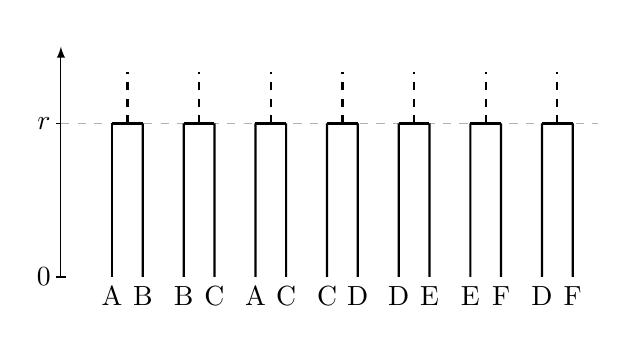
\begin{tikzpicture}[scale=0.65]
            
            % Hauteur de l'axe Y correspondant au niveau de fusion "r"
            \def\h{3.0}
            
            % Axe vertical pour localiser clairement la valeur r
            \draw[->, >=latex] (-1, 0) -- (-1, \h+1.5) node[above] {};
            \draw (-1.1, \h) -- (-0.9, \h) node[left=2pt] {$r$};
            \draw (-1.1, 0) -- (-0.9, 0) node[left=2pt] {$0$};
            
            % Ligne horizontale pointillée pour lier visuellement toutes les fusions à la hauteur r
            \draw[dashed, gray!60] (-1, \h) -- (9.5, \h);
            
            % Boucle générant la forêt des 7 fusions indépendantes
            % count=\i permet d'espacer mathématiquement chaque arbre sur l'axe X (0, 1.4, 2.8...)
            \foreach \L/\R [count=\i] in {A/B, B/C, A/C, C/D, D/E, E/F, D/F} {
                
                % Espacement horizontal entre les sous-dendrogrammes
                \pgfmathsetmacro{\x}{(\i-1)*1.4}
                
                % Coordonnées des feuilles
                \coordinate (L\i) at (\x, 0);
                \coordinate (R\i) at (\x+0.6, 0);
                
                % Affichage des lettres en bas
                \node[below] at (L\i) {\L};
                \node[below] at (R\i) {\R};
                
                % Lignes verticales montantes depuis les feuilles jusqu'au niveau r
                \draw[thick] (L\i) -- (\x, \h);
                \draw[thick] (R\i) -- (\x+0.6, \h);
                
                % Barre de fusion horizontale (le pont) au niveau r
                \draw[thick] (\x, \h) -- (\x+0.6, \h);
                
                % Pointillés verticaux montant depuis le milieu de la fusion
                % Ils indiquent que l'arbre complet continue de se construire au-dessus
                \draw[thick, dashed] (\x+0.3, \h) -- (\x+0.3, \h+1.0);
            }
            
        \end{tikzpicture}
        \caption{Fusions des sept segments au niveau $r$}
        \label{fig:foret_dendrogrammes}
    \end{subfigure}
    
    \caption{Gauche : nuage $\mathcal X$ repris de la \Fig~\ref{fig:nuage} avec en bleu les amas de forte densité au niveau $r' \gtrsim r$. Droite : le dendrogramme en construction. Par convention, le multi-ensemble des feuilles apparaît au niveau $0$. Au niveau $r$, les sept amas correspondant aux sept segments apparaissent.}
    \label{fig:complexe_rprime}
\end{figure}


Pour $K=2$, les premiers amas de forte densité apparaissent au niveau $r$ (\emph{cf}. la \Fig~\ref{fig:intersections_rprime}). Il sont au nombre de sept et en correspondance avec les sept segments de longueur $2r$ (\Fig~\ref{fig:foret_dendrogrammes}).


\begin{figure}[htbp]
    \centering
    
    % ---------------------------------------------------
    % SOUS-FIGURE (a) : Intersections au seuil r' exact
    % ---------------------------------------------------
    \begin{subfigure}[b]{0.45\textwidth}
        \centering
        \begin{tikzpicture}[scale=0.55]
            
            % r est la moitié du segment
            \def\r{1.5}
            
            % r' est calculé mathématiquement pour que les 3 cercles s'intersectent 
            % en 1 point central. Pour un triangle équilatéral de côté 2r, 
            % le rayon circonscrit est r' = 2r / sqrt(3).
            \pgfmathsetmacro{\rprime}{\r * 2 / sqrt(3)}
            
            % 1. Appel du template
            \templateNuage[\r]
            
            % 2. Dessin en arrière-plan
            \begin{scope}[on background layer]
                
                % Remplissage bleu foncé des intersections deux à deux
                % La superposition génère d'elle-même une zone un peu plus sombre
                % au centre où les 3 lentilles se chevauchent.
                \foreach \p/\q in {A/B, B/C, C/A, C/D, D/E, E/F, F/D} {
                    \begin{scope}
                        \clip (\p) circle (\rprime);
                        \fill[blue!60!black, opacity=0.4] (\q) circle (\rprime);
                    \end{scope}
                }
                
                % Tracé des 6 cercles de rayon r' (en pointillés gris)
                \foreach \P in {A,B,C,D,E,F} {
                    \draw[dashed, thick, gray!80] (\P) circle (\rprime);
                }
                
            \end{scope}
            
            % 3. Ajout des points rouges au centre des triangles 
            % Utilisation des coordonnées barycentriques de TikZ pour trouver le centre exact
            \fill[red] (barycentric cs:A=1,B=1,C=1) circle (3.5pt);
            \fill[red] (barycentric cs:D=1,E=1,F=1) circle (3.5pt);
            
            % 4. Flèche indiquant r' (orientée vers le haut-gauche)
            \draw[>=latex] (A) -- ++(135:\rprime) node[midway, sloped, above] {$r'$};
            
        \end{tikzpicture}
        \caption{$3$-intersection (rouge) pour $r' = \frac{2\sqrt{3}}{3}r$}
        \label{fig:intersections_rprime_exact}
    \end{subfigure}
    \hfill
    % ---------------------------------------------------
    % SOUS-FIGURE (b) : Dendrogrammes avec fusions à r et r'
    % ---------------------------------------------------
    \begin{subfigure}[b]{0.53\textwidth}
        \centering
        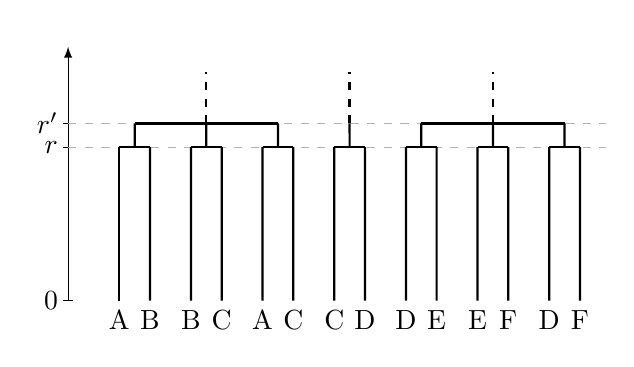
\begin{tikzpicture}[scale=0.65]
            
            % Hauteurs des niveaux de fusion
            \def\hr{3}      % Hauteur du niveau r
            \def\hrprime{3.46410161514} % Hauteur du niveau r'
            
            % Axe vertical des niveaux
            \draw[->, >=latex] (-1, 0) -- (-1, \hrprime+1.5) node[above] {};
            \draw (-1.1, \hr) -- (-0.9, \hr) node[left=2pt] {$r$};
            \draw (-1.1, \hrprime) -- (-0.9, \hrprime) node[left=2pt] {$r'$};
            \draw (-1.1, 0) -- (-0.9, 0) node[left=2pt] {$0$};
            
            % Lignes horizontales guides en pointillés
            \draw[dashed, gray!60] (-1, \hr) -- (9.5, \hr);
            \draw[dashed, gray!60] (-1, \hrprime) -- (9.5, \hrprime);
            
            % ==============================================
            % 1. BASE DU DENDROGRAMME : Fusions à r
            % ==============================================
            \foreach \L/\R [count=\i] in {A/B, B/C, A/C, C/D, D/E, E/F, D/F} {
                
                \pgfmathsetmacro{\x}{(\i-1)*1.4}
                \coordinate (L\i) at (\x, 0);
                \coordinate (R\i) at (\x+0.6, 0);
                
                % M\i représente le point central du pont de la fusion à r
                \coordinate (M\i) at (\x+0.3, \hr); 
                
                \node[below] at (L\i) {\L};
                \node[below] at (R\i) {\R};
                
                \draw[thick] (L\i) -- (\x, \hr);
                \draw[thick] (R\i) -- (\x+0.6, \hr);
                \draw[thick] (\x, \hr) -- (\x+0.6, \hr);
                
                % Prolongement vertical du tronc qui résulte de la fusion jusqu'à r'
                \draw[thick] (M\i) -- (\x+0.3, \hrprime);
            }
            
            % ==============================================
            % 2. ÉTAGE SUPÉRIEUR : Nouvelles fusions à r'
            % ==============================================
            
            % --- Fusion du triangle gauche (arêtes 1, 2, 3) ---
            % Leurs troncs arrivent aux abscisses 0.3, 1.7 et 3.1
            \draw[thick] (0.3, \hrprime) -- (3.1, \hrprime); % Pont horizontal qui relie les trois
            \draw[thick, dashed] (1.7, \hrprime) -- (1.7, \hrprime+1.0); % Le tronc commun en pointillés
            
            % --- Arête centrale C-D qui ne fusionne pas (arête 4) ---
            % Son tronc arrive à l'abscisse 4.5
            \draw[thick, dashed] (4.5, \hrprime) -- (4.5, \hrprime+1.0); % Continue de monter seule
            
            % --- Fusion du triangle droit (arêtes 5, 6, 7) ---
            % Leurs troncs arrivent aux abscisses 5.9, 7.3 et 8.7
            \draw[thick] (5.9, \hrprime) -- (8.7, \hrprime); % Pont horizontal qui relie les trois
            \draw[thick, dashed] (7.3, \hrprime) -- (7.3, \hrprime+1.0); % Le tronc commun en pointillés
            
        \end{tikzpicture}
        \caption{Fusions de dimension supérieure à $r'$}
        \label{fig:fusion_rprime}
    \end{subfigure}
    
    \caption{Évolution des amas de forte densité $K$-NN avec $K=2$ au niveau $r' = \frac{2\sqrt{3}}{3}r$. Gauche : on voit apparaître des fusions de $2$-intersections de boules au moyen de $3$-intersections (le point de contact de la fusion est repéré en rouge). Droite : l'évolution du dendrogramme hiérarchique avec les fusions opérées au niveau $r'$.}
    \label{fig:complexe_rprime_exact}
\end{figure}

Au niveau $r' = \frac{2\sqrt{3}}{3}r$, des $3$-intersections de boules apparaissent fusionnant certains amas de forte densité. Voir la \Fig~\ref{fig:complexe_rprime_exact} pour plus de détails.



\begin{figure}[htbp]
    \centering
    
    % ---------------------------------------------------
    % SOUS-FIGURE (a) : Intersections au seuil r'' = AD/2
    % ---------------------------------------------------
    \begin{subfigure}[b]{0.48\textwidth}
        \centering
        \begin{tikzpicture}[scale=0.45]
            
            \def\r{1.5}
            
            % r'' = AD/2. La formule mathématique exacte :
            \pgfmathsetmacro{\rsecond}{\r * sqrt(2 + sqrt(3))}
            
            % 1. Appel du template modifié au premier plan
            \templateNuage[\r]
            
            % 2. Dessin des intersections sous le graphe (arrière-plan)
            \begin{scope}[on background layer]
                
                % -- 2-INTERSECTIONS (Bleu foncé surfacique) --
                \foreach \p/\q in {A/B, B/C, C/A, C/D, D/E, E/F, F/D} {
                    \begin{scope}
                        \clip (\p) circle (\rsecond);
                        \fill[blue!60!black, opacity=0.25] (\q) circle (\rsecond);
                    \end{scope}
                }
                
                % -- 3-INTERSECTIONS (Rouge pur) --
                % Triangle gauche (A, B, C)
                \begin{scope}
                    \clip (A) circle (\rsecond);
                    \clip (B) circle (\rsecond);
                    \clip (C) circle (\rsecond);
                    % On efface le bleu sous-jacent avec du blanc, puis on remplit en rouge
                    \fill[white] (-10,-10) rectangle (10,10); 
                    \fill[red, opacity=0.6] (-10,-10) rectangle (10,10);
                \end{scope}
                
                % Triangle droit (D, E, F)
                \begin{scope}
                    \clip (D) circle (\rsecond);
                    \clip (E) circle (\rsecond);
                    \clip (F) circle (\rsecond);
                    \fill[white] (-10,-10) rectangle (10,10); 
                    \fill[red, opacity=0.6] (-10,-10) rectangle (10,10);
                \end{scope}
                
                % Tracé des 6 grands cercles originaux (pointillés gris)
                \foreach \P in {A,B,C,D,E,F} {
                    \draw[dashed, thick, gray!60] (\P) circle (\rsecond);
                }
                
            \end{scope}
            
            % 3. Ajout didactique des 4 points de tangence simultanés (en rouge)
            % Calculés par TikZ avec une précision absolue au milieu des segments croisés
            \fill[red] ($ (A)!0.5!(D) $) circle (3.5pt); % Tangence A-D (Haut côté C)
            \fill[red] ($ (C)!0.5!(E) $) circle (3.5pt); % Tangence C-E (Haut côté D)
            \fill[red] ($ (B)!0.5!(D) $) circle (3.5pt); % Tangence B-D (Bas côté C)
            \fill[red] ($ (C)!0.5!(F) $) circle (3.5pt); % Tangence C-F (Bas côté D)
            
            % Flèche indiquant le rayon r'' (dirigée vers l'extérieur pour ne rien masquer)
            \draw[>=latex] (A) -- ++(135:\rsecond) node[midway, sloped, above=1pt] {$r''$};
            
        \end{tikzpicture}
        \caption{Connexité globale atteinte pour $r''=AD/2$}
        \label{fig:intersections_rsecond}
    \end{subfigure}
    \hfill
    % ---------------------------------------------------
    % SOUS-FIGURE (b) : Dendrogramme final complet
    % ---------------------------------------------------
    \begin{subfigure}[b]{0.51\textwidth}
        \centering
        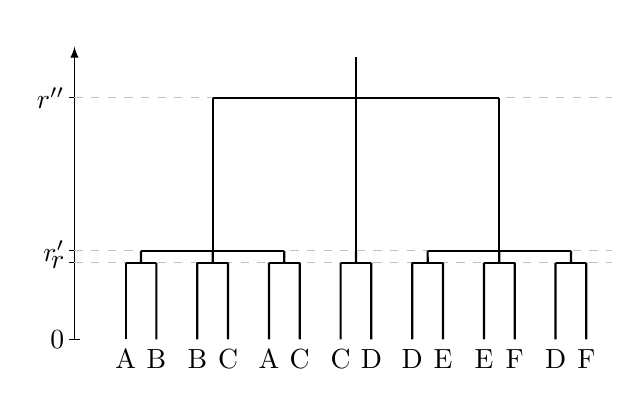
\begin{tikzpicture}[scale=0.65]
            
            % Hauteurs successives des 3 niveaux de fusion
            \def\hr{1.5}       % Niveau r
            \def\hrprime{1.732}  % Niveau r' 1.5 * 2/3 \sqrt{3}
            \def\hrsecond{4.72} % Niveau r'' 1.5*(\sqrt{3}+\sqrt{2})
            %\pgfmathsetmacro{\rsecond}{\r * sqrt(2 + sqrt(3))}
            
            % Axe vertical
            \draw[->, >=latex] (-1, 0) -- (-1, \hrsecond+1.0) node[above] {};
            \draw (-1.1, \hr) -- (-0.9, \hr) node[left=2pt] {$r$};
            \draw (-1.1, \hrprime) -- (-0.9, \hrprime) node[left=2pt] {$r'$};
            \draw (-1.1, \hrsecond) -- (-0.9, \hrsecond) node[left=2pt] {$r''$};
            \draw (-1.1, 0) -- (-0.9, 0) node[left=2pt] {$0$};
            
            % Lignes guides horizontales
            \draw[dashed, gray!50] (-1, \hr) -- (9.5, \hr);
            \draw[dashed, gray!50] (-1, \hrprime) -- (9.5, \hrprime);
            \draw[dashed, gray!50] (-1, \hrsecond) -- (9.5, \hrsecond);
            
            % ==============================================
            % NIVEAU 1 : Fusions initiales à r
            % ==============================================
            \foreach \L/\R [count=\i] in {A/B, B/C, A/C, C/D, D/E, E/F, D/F} {
                \pgfmathsetmacro{\x}{(\i-1)*1.4}
                \coordinate (L\i) at (\x, 0);
                \coordinate (R\i) at (\x+0.6, 0);
                \coordinate (M\i) at (\x+0.3, \hr); 
                
                \node[below] at (L\i) {\L};
                \node[below] at (R\i) {\R};
                
                \draw[thick] (L\i) -- (\x, \hr);
                \draw[thick] (R\i) -- (\x+0.6, \hr);
                \draw[thick] (\x, \hr) -- (\x+0.6, \hr);
                
                % Les 7 troncs montent jusqu'au niveau r'
                \draw[thick] (M\i) -- (\x+0.3, \hrprime);
            }
            
            % ==============================================
            % NIVEAU 2 : Fusions des sous-composantes à r'
            % ==============================================
            % Tronc gauche (fusion du triangle ABC)
            \draw[thick] (0.3, \hrprime) -- (3.1, \hrprime);
            \draw[thick] (1.7, \hrprime) -- (1.7, \hrsecond);
            
            % Tronc droit (fusion du triangle DEF)
            \draw[thick] (5.9, \hrprime) -- (8.7, \hrprime);
            \draw[thick] (7.3, \hrprime) -- (7.3, \hrsecond);
            
            % Arête centrale 4 (C/D) qui traverse r' sans fusionner
            \draw[thick] (4.5, \hrprime) -- (4.5, \hrsecond); 
            
            % ==============================================
            % NIVEAU 3 : Fusion finale globale à r''
            % ==============================================
            % On unifie le tronc gauche (x=1.7), le tronc central (x=4.5) et le tronc droit (x=7.3)
            \draw[thick] (1.7, \hrsecond) -- (7.3, \hrsecond);
            
            % Racine finale du dendrogramme (Single-Linkage) en trait PLEIN
            \draw[thick] (4.5, \hrsecond) -- (4.5, \hrsecond+0.8);
            
        \end{tikzpicture}
        \caption{Clôture du dendrogramme à $r''$}
        \label{fig:fusion_rsecond}
    \end{subfigure}
    
    \caption{Clôture de la hiérarchie $2$-NN au niveau $r'' = AD/2$. À ce rayon critique, l'apparition simultanée des quatre points de tangence (points rouges) relient les trois amas de forte densité.}
    \label{fig:complexe_rsecond}
\end{figure}

Enfin, au niveau $r''= \frac{AD}{2}$, des jonctions apparaissent entre les trois amas de forte densité du niveau, clôturant ainsi le dendrogramme. Voir la \Fig~\ref{fig:complexe_rsecond}.


Comme déjà esquissé dans la première partie, l'on s'aperçoit que pour rendre compte des $K \ge 2$ plus proches voisins, il va être nécessaire de relâcher l'hypothèse d'un clustering vu comme une partition sur les données $\mathcal X$.
Les interaction d'ordre supérieur (ici des arêtes connectées entre elles au moyen de triangles\footnote{C'est pourquoi le seuil de connexion global $r'' = AD/2$ : à ce niveau, le triangle ACD apparaît connectant les arêtes AC et CD.}).


\Synthese{Ce chapitre de transition entre la présentation du Single-Linkage, ses descendants actuels tels que HDBSCAN, et la généralisation que nous en proposons dans les chapitres suivants, a pour but de montrer au lecteur les limites des algorithmes actuels\footnote{L'on aurait pu aussi citer les auteurs de \cite{GeneralizedSL}, qui construisent un graphe géométrique sur les données puis échantillonnent la densité le long de ses arêtes.} et donner l'intuition de l'algorithme que nous proposons ci-dessous.}